\documentclass[10pt]{beamer}
\usepackage{../sty/nmf-ps-talk}
\title{Identifying Textual Clusters\\with Non-negative Matrix Factorization}
\author{Joey McCollum\inst{*}}
\institute{\inst{*}Virginia Polytechnic Institute and State University}
\date{16 September 2020}
\begin{document}
	\begin{frame}
		\titlepage
		\phantom{\cite{Swanson.Luke}\cite{Lin16}\cite{CT69}\cite{Colwell69}\cite{Epp12}\cite{Wisse82}\cite{GS00}\cite{Wasserman06}\cite{McCollum19}\cite{BTGM04}\cite{Geer94}\cite{Zuntz53},\cite{Colwell32}\cite{Amphoux81}\cite{SWH02}\cite{Morrill12}\cite{Jones72}\cite{Lake02}\cite{LL41}\cite{Geerlings.Matthew}\cite{Geerlings.Luke}\cite{Geerlings.John}}
	\end{frame}
	\begin{frame}{How Do We Compare Manuscripts?}
		\begin{itemize}
			\item Start with collation—aligning texts at \emph{variation units}
		\end{itemize}
		\begin{center}
			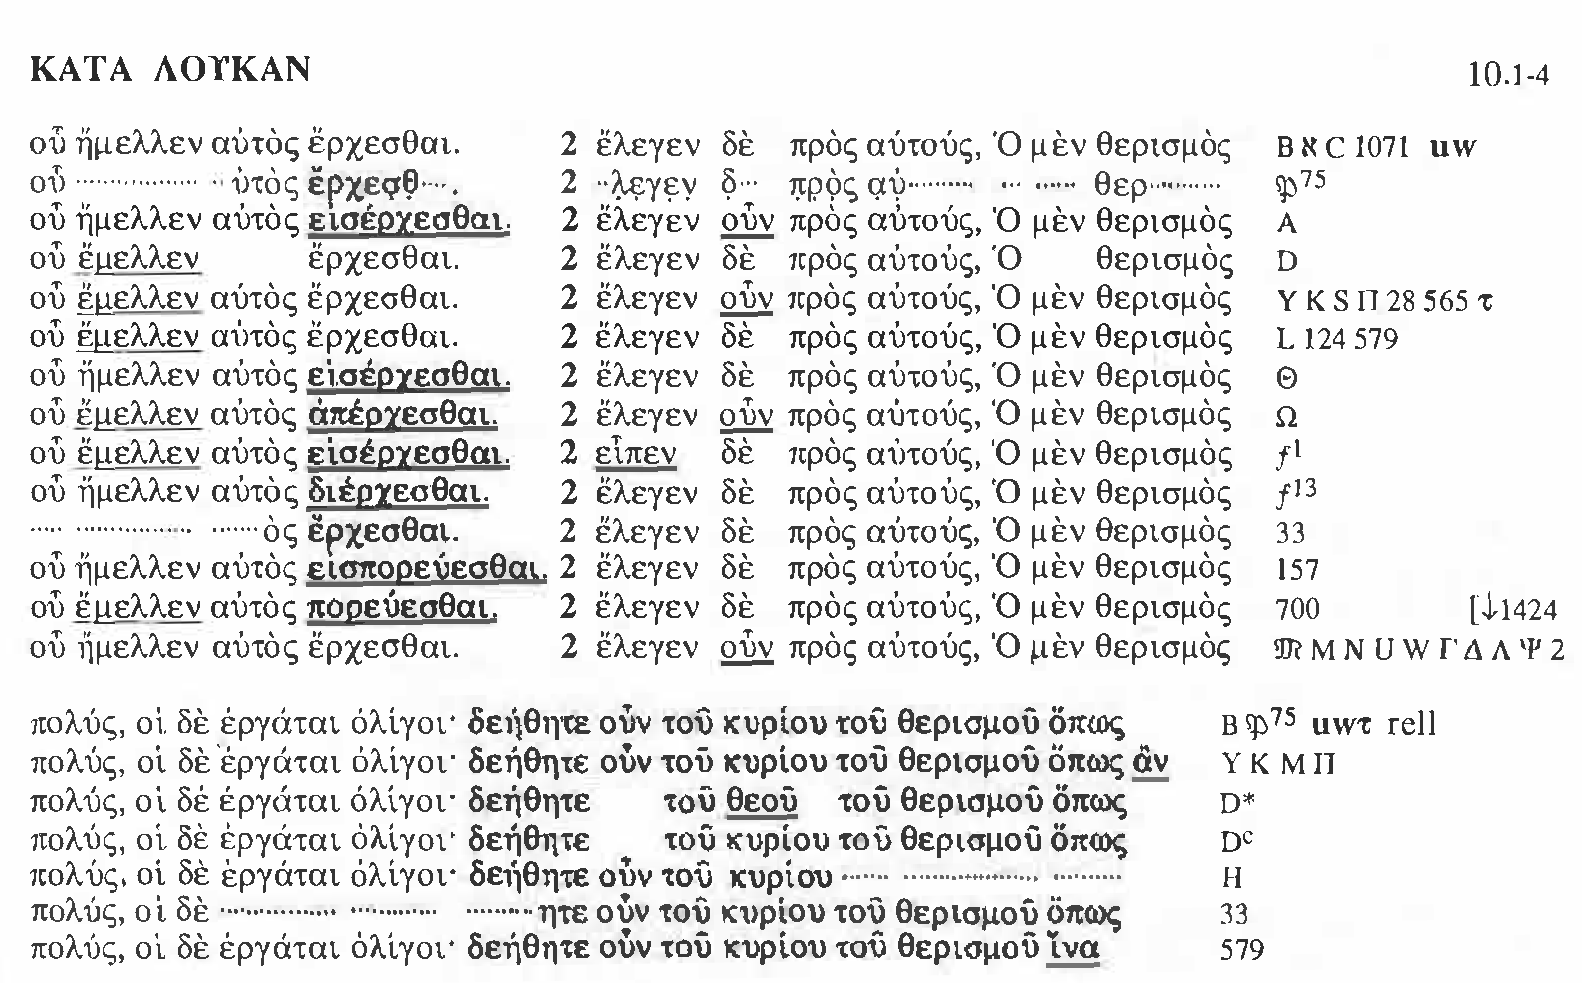
\includegraphics[width=0.75\textwidth]{../graphics/swanson_scan_luke_10_2.png}
		\end{center}
		\footnotesize\parencite[Source:][183]{Swanson.Luke}
	\end{frame}
	\begin{frame}{How Do We Compare Manuscripts?}
		\begin{itemize}
			\item Start with collation—aligning texts at \emph{variation units}
		\end{itemize}
		\begin{center}
			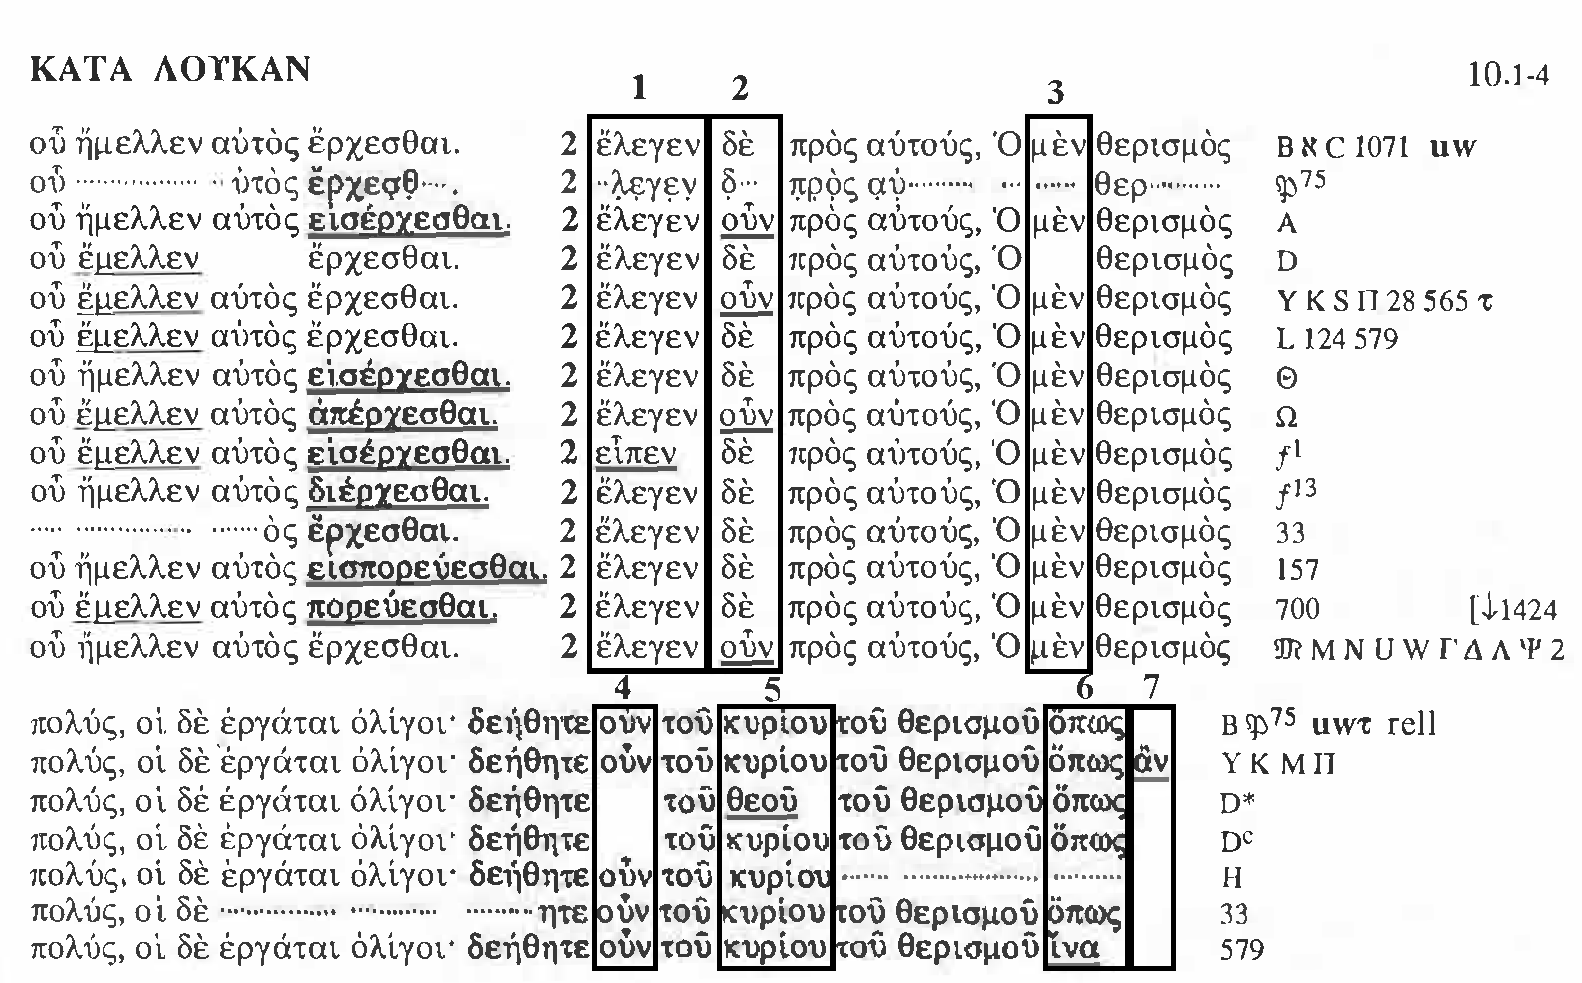
\includegraphics[width=0.75\textwidth]{../graphics/swanson_scan_luke_10_2_variation_units.png}
		\end{center}
		\phantom{\footnotesize\parencite[Source:][183]{Swanson.Luke}}
	\end{frame}
	\begin{frame}{How Do We Compare Manuscripts?}
		\begin{itemize}
			\item Comparable to DNA sequence alignment\footnote{For the fascinating history of this relationship, see \cite{Lin16}.}
			\begin{itemize}
				\item manuscripts $\longleftrightarrow$ taxa / species
				\item variation units $\longleftrightarrow$ sites
				\item variant readings $\longleftrightarrow$ bases (A, C, G, T) and gaps (–)
			\end{itemize}
		\end{itemize}
		\begin{center}
			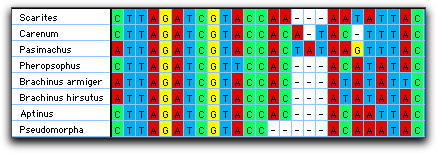
\includegraphics[width=\textwidth]{../graphics/sequence_alignment.jpg}
			
			\footnotesize(Source: \url{http://www.sequence-alignment.com})
		\end{center}	
	\end{frame}
	\begin{frame}{How Do We Compare Manuscripts?}
		\begin{itemize}
			\item This provides a simple basis of comparison between pairs of manuscripts
			\begin{itemize}
				\item Number of units where both agree
				\item For a proportion, divide by number of units where the readings of both are known
			\end{itemize}
			\item ``Pre-genealogical coherence'' in the Coherence-Based Genealogical Method (CBGM)
		\end{itemize}
		\begin{center}
			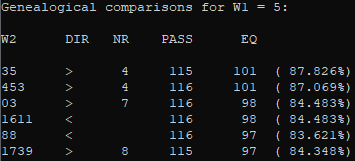
\includegraphics[width=0.5\textwidth]{../graphics/compare_witnesses.png}
		\end{center}
		\begin{itemize}
			\item Can we use mutual agreement to classify manuscripts into groups?
		\end{itemize}
	\end{frame}
	\begin{frame}{The Quantitative Method}
		\begin{itemize}
			\item Colwell and Tune: if manuscripts agree significantly more with one another than they do with other manuscripts, then they form a family, or \emph{text-type}\footnote{\cite{CT69}.}
			\begin{itemize}
				\item $\geq 70\%$ with one another, and $\geq 10\%$ more than with others
			\end{itemize}
		\end{itemize}
		\begin{center}
			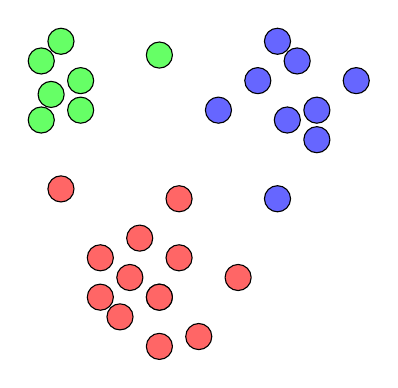
\begin{tikzpicture}
			%Green cluster:
			\path
				(0.0, 3.75) node[shape=circle, draw=black, fill=green!60, scale=1.0 ] {}
				(0.25, 4.0) node[shape=circle, draw=black, fill=green!60, scale=1.0 ] {}
				(0.125, 3.325) node[shape=circle, draw=black, fill=green!60, scale=1.0 ] {}
				(0.5, 3.125) node[shape=circle ,draw=black, fill=green!60, scale=1.0 ] {}
				(0.0, 3.0) node[shape=circle, draw=black, fill=green!60, scale=1.0 ] {}
				(0.5, 3.5) node[shape=circle, draw=black, fill=green!60, scale=1.0 ] {}
				(1.5, 3.825) node[shape=circle, draw=black, fill=green!60, scale=1.0 ] {};
			%Blue cluster:
			\path
				(2.25, 3.125) node[shape=circle, draw=black, fill=blue!60, scale=1.0 ] {}
				(3.0, 4.0) node[shape=circle, draw=black, fill=blue!60, scale=1.0 ] {}
				(3.25, 3.75) node[shape=circle, draw=black, fill=blue!60, scale=1.0 ] {}
				(3.125, 3.0) node[shape=circle, draw=black, fill=blue!60, scale=1.0 ] {}
				(3.5, 3.125) node[shape=circle ,draw=black, fill=blue!60, scale=1.0 ] {}
				(2.75, 3.5) node[shape=circle, draw=black, fill=blue!60, scale=1.0 ] {}
				(3.5, 2.75) node[shape=circle, draw=black, fill=blue!60, scale=1.0 ] {}
				(4.0, 3.5) node[shape=circle, draw=black, fill=blue!60, scale=1.0 ] {}
				(3.0, 2.0) node[shape=circle, draw=black, fill=blue!60, scale=1.0 ] {};
			%Red cluster:
			\path
				(0.25, 2.125) node[shape=circle, draw=black, fill=red!60, scale=1.0 ] {}
				(0.75, 1.25) node[shape=circle, draw=black, fill=red!60, scale=1.0 ] {}
				(0.75, 0.75) node[shape=circle, draw=black, fill=red!60, scale=1.0 ] {}
				(1.5, 0.75) node[shape=circle, draw=black, fill=red!60, scale=1.0 ] {}
				(1.75, 2.0) node[shape=circle, draw=black, fill=red!60, scale=1.0 ] {}
				(1.125, 1.0) node[shape=circle, draw=black, fill=red!60, scale=1.0 ] {}
				(1.5, 0.125) node[shape=circle ,draw=black, fill=red!60, scale=1.0 ] {}
				(1.0, 0.5) node[shape=circle, draw=black, fill=red!60, scale=1.0 ] {}
				(1.25, 1.5) node[shape=circle, draw=black, fill=red!60, scale=1.0 ] {}
				(1.5, 0.75) node[shape=circle, draw=black, fill=red!60, scale=1.0 ] {}
				(1.75, 1.25) node[shape=circle, draw=black, fill=red!60, scale=1.0 ] {}
				(2.0, 0.25) node[shape=circle, draw=black, fill=red!60, scale=1.0 ] {}
				(2.5, 1.0) node[shape=circle, draw=black, fill=red!60, scale=1.0 ] {};
			\end{tikzpicture}
		\end{center}
	\end{frame}
	\begin{frame}{The Quantitative Method}
		\begin{itemize}
			\item Problems:
			\begin{itemize}
				\item All units (including those involving singular readings and common scribal errors) have equal weight
				\item Mixture in the transmission process is a problem\footnote{\cite{Epp12}.}
			\end{itemize}
		\end{itemize}
		\begin{center}
			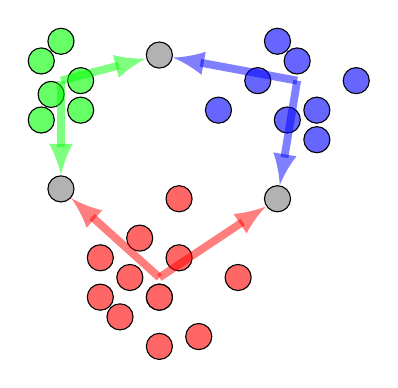
\begin{tikzpicture}
			%Green cluster:
			\path
				(0.0, 3.75) node[shape=circle, draw=black, fill=green!60, scale=1.0 ] {}
				(0.25, 4.0) node[shape=circle, draw=black, fill=green!60, scale=1.0 ] {}
				(0.125, 3.325) node[shape=circle, draw=black, fill=green!60, scale=1.0 ] {}
				(0.5, 3.125) node[shape=circle ,draw=black, fill=green!60, scale=1.0 ] {}
				(0.0, 3.0) node[shape=circle, draw=black, fill=green!60, scale=1.0 ] {}
				(0.5, 3.5) node[shape=circle, draw=black, fill=green!60, scale=1.0 ] {}
				(1.5, 3.825) node[shape=circle, draw=black, fill=gray!60, scale=1.0 ] (gray1) {};
			%Blue cluster:
			\path
				(2.25, 3.125) node[shape=circle, draw=black, fill=blue!60, scale=1.0 ] {}
				(3.0, 4.0) node[shape=circle, draw=black, fill=blue!60, scale=1.0 ] {}
				(3.25, 3.75) node[shape=circle, draw=black, fill=blue!60, scale=1.0 ] {}
				(3.125, 3.0) node[shape=circle, draw=black, fill=blue!60, scale=1.0 ] {}
				(3.5, 3.125) node[shape=circle ,draw=black, fill=blue!60, scale=1.0 ] {}
				(2.75, 3.5) node[shape=circle, draw=black, fill=blue!60, scale=1.0 ] {}
				(3.5, 2.75) node[shape=circle, draw=black, fill=blue!60, scale=1.0 ] {}
				(4.0, 3.5) node[shape=circle, draw=black, fill=blue!60, scale=1.0 ] {}
				(3.0, 2.0) node[shape=circle, draw=black, fill=gray!60, scale=1.0 ] (gray2) {};
			%Red cluster:
			\path
				(0.25, 2.125) node[shape=circle, draw=black, fill=gray!60, scale=1.0 ] (gray3) {}
				(0.75, 1.25) node[shape=circle, draw=black, fill=red!60, scale=1.0 ] {}
				(0.75, 0.75) node[shape=circle, draw=black, fill=red!60, scale=1.0 ] {}
				(1.5, 0.75) node[shape=circle, draw=black, fill=red!60, scale=1.0 ] {}
				(1.75, 2.0) node[shape=circle, draw=black, fill=red!60, scale=1.0 ] {}
				(1.125, 1.0) node[shape=circle, draw=black, fill=red!60, scale=1.0 ] {}
				(1.5, 0.125) node[shape=circle ,draw=black, fill=red!60, scale=1.0 ] {}
				(1.0, 0.5) node[shape=circle, draw=black, fill=red!60, scale=1.0 ] {}
				(1.25, 1.5) node[shape=circle, draw=black, fill=red!60, scale=1.0 ] {}
				(1.5, 0.75) node[shape=circle, draw=black, fill=red!60, scale=1.0 ] {}
				(1.75, 1.25) node[shape=circle, draw=black, fill=red!60, scale=1.0 ] {}
				(2.0, 0.25) node[shape=circle, draw=black, fill=red!60, scale=1.0 ] {}
				(2.5, 1.0) node[shape=circle, draw=black, fill=red!60, scale=1.0 ] {};
			%Mixture arrows:
			\draw[->, >=latex,line width=0.1cm, color=green, opacity=0.5]
				(0.25, 3.5) -- (gray1);
			\draw[->, >=latex,line width=0.1cm, color=blue, opacity=0.5]
				(3.25, 3.5) -- (gray1);
			\draw[->, >=latex,line width=0.1cm, color=red, opacity=0.5]
				(1.5, 1.0) -- (gray2);
			\draw[->, >=latex,line width=0.1cm, color=blue, opacity=0.5]
				(3.25, 3.5) -- (gray2);
			\draw[->, >=latex,line width=0.1cm, color=red, opacity=0.5]
				(1.5, 1.0) -- (gray3);
			\draw[->, >=latex,line width=0.1cm, color=green, opacity=0.5]
				(0.25, 3.5) -- (gray3);
			\end{tikzpicture}
		\end{center}
	\end{frame}
	\begin{frame}{The Quantitative Method}
		\begin{itemize}
			\item For efficiency and accuracy, comparisons should be done on the basis of \emph{informative} points of variation\footnote{\cite{Colwell69}.}
			\item Specific readings, not the variation units containing them
			\item But how do we know which ones are the most informative?
			\begin{center}
				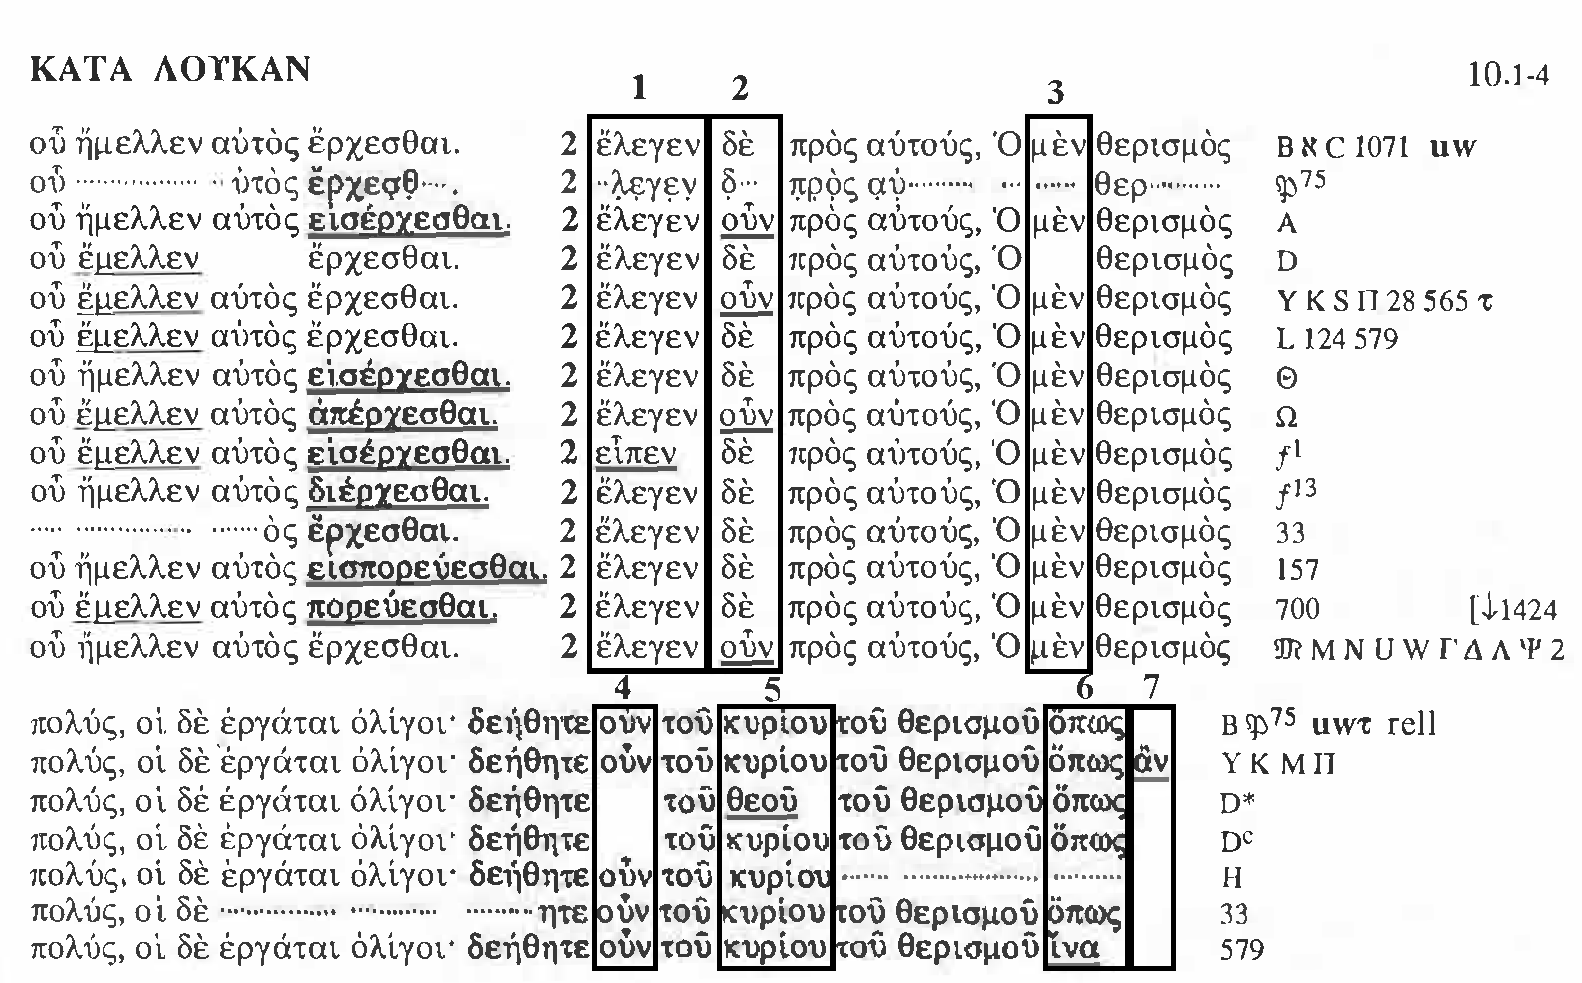
\includegraphics[width=0.75\textwidth]{../graphics/swanson_scan_luke_10_2_variation_units.png}
			\end{center}
		\end{itemize}
	\end{frame}
	\begin{frame}{The Claremont Profile Method}
		\begin{itemize}
			\item Start with an established set of manuscript groups\footnote{\cite{Wisse82}.}
			\item Filter out variation units involving common types of variation and singular / subsingular readings to get a set of \emph{test passages}
			\item Readings supported by group manuscripts = the group's \emph{profile}
		\end{itemize}
		\begin{center}
			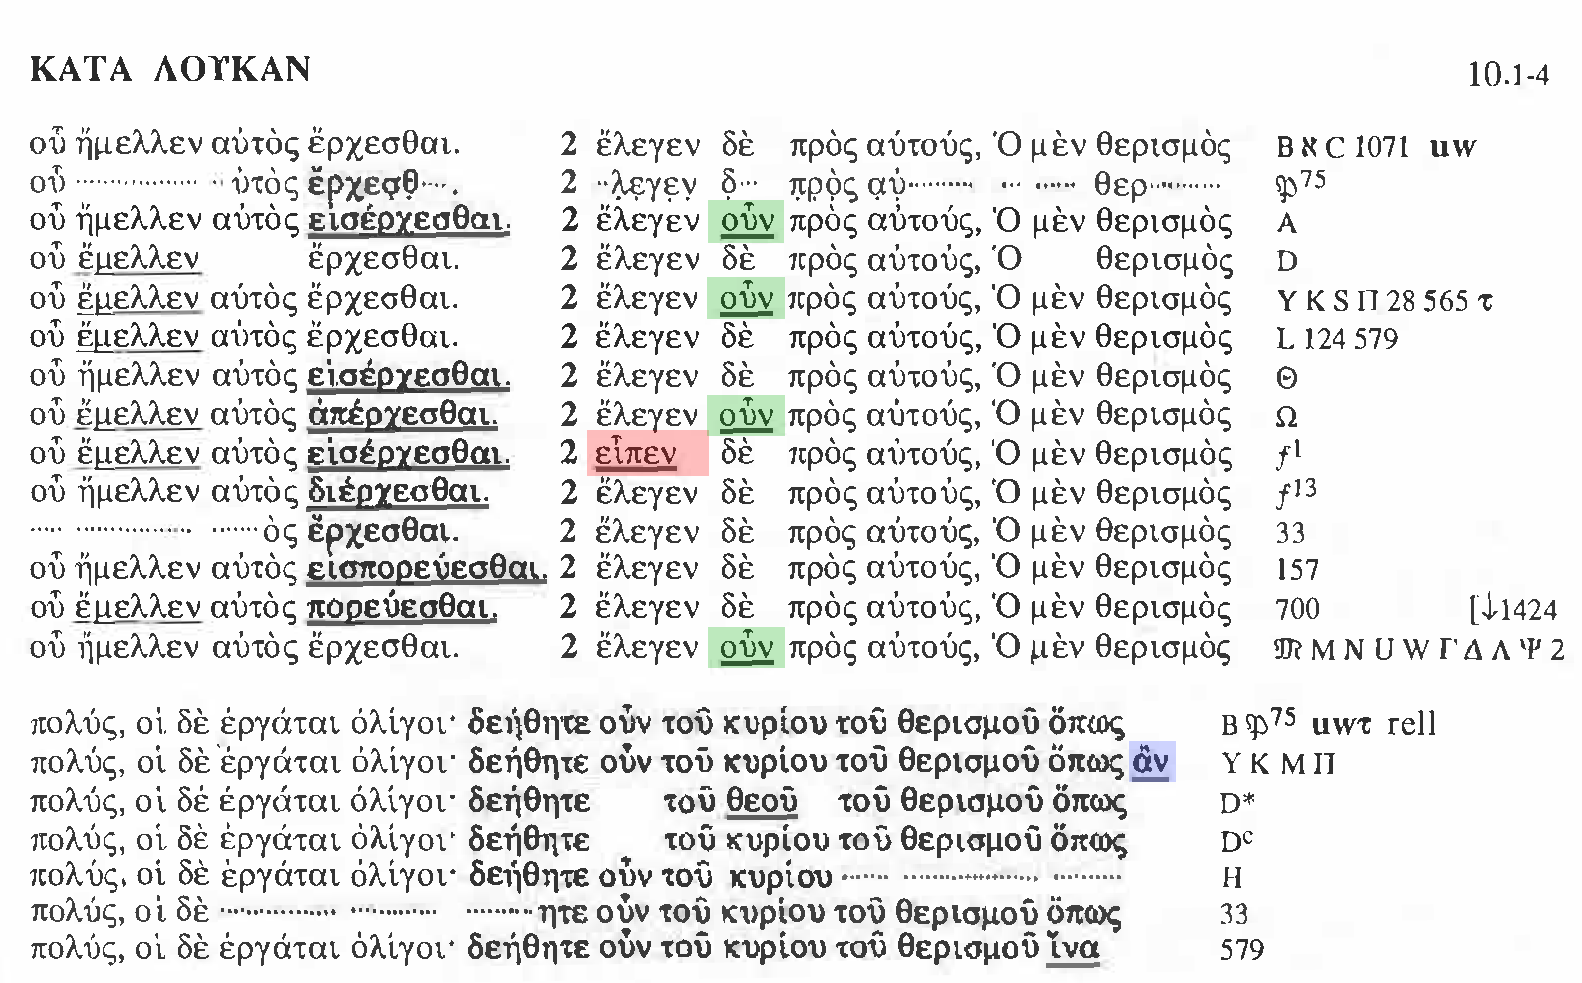
\includegraphics[width=0.75\textwidth]{../graphics/swanson_scan_luke_10_2_cpm.png}
		\end{center}
	\end{frame}
	\begin{frame}{The Claremont Profile Method}
		\begin{itemize}
			\item This allows us to isolate informative readings for group classification
			\item Also robust to mixture
			\item But it needs manuscript groups to be established first!
			\item ``Good manuscripts have good readings, and good readings are found in good manuscripts''
		\end{itemize}
		\begin{center}
			\begin{tikzpicture}
				%Nodes:
				\node[cloud, cloud puffs=13, cloud ignores aspect, minimum width=3cm, minimum height=2cm, align=center,fill=white, draw, very thick] (mss)  at (0, 2.5) {Group\\Manuscripts};
				\node[cloud, cloud puffs=13, cloud ignores aspect, minimum width=3cm, minimum height=2cm, align=center, fill=white, draw, very thick] (rdgs) at (0, 0) {Group\\Readings};
				%Edges:
				\draw[->, >=latex, very thick] (mss.east) to[bend left] (rdgs.east);
				\draw[->, >=latex, very thick] (rdgs.west) to[bend left] (mss.west);
			\end{tikzpicture}
		\end{center}
	\end{frame}
	\begin{frame}{Non-negative Matrix Factorization}
		\begin{itemize}
			\item \emph{Non-negative matrix factorization} (NMF), a machine learning technique, uses this circular relationship to solve both problems
		\end{itemize}
		\begin{columns}[T]
			\begin{column}{0.3\textwidth}
				\begin{itemize}
					\item Represent our collation as a matrix $\mathbf{A}$ with a row for each variant reading and a column for each manuscript
					\item $m$ rows by $n$ columns
				\end{itemize}
			\end{column}
			\begin{column}{0.6\textwidth}
				\matrixfont
				\footnotesize
				\setlength{\tabcolsep}{5pt}
				\begin{tabular}{ll|rrrrrrr}
					 & & $\mathfrak{P}$\textsuperscript{75}& A & B & D & K & \emph{f}\textsuperscript{1} & 579\\
					\hline
					\multirow{2}{*}{Unit 1} & ἔλεγεν & 1 & 1 & 1 & 1 & 1 & 0 & 1\\
					& εἶπεν & 0 & 0 & 0 & 0 & 0 & 1 & 0\\
					\hline
					\multirow{2}{*}{Unit 2} & δὲ & 1 & 0 & 1 & 1 & 0 & 1 & 1\\
					 & οὖν & 0 & 1 & 0 & 0 & 1 & 0 & 0\\
					\hline
					\multirow{2}{*}{Unit 3} & μὲν & 0 & 1 & 1 & 0 & 1 & 1 & 1\\
					 & \emph{omit} & 0 & 0 & 0 & 1 & 0 & 0 & 0\\
					\hline
					\multirow{2}{*}{Unit 4} & οὖν & 1 & 1 & 1 & 0 & 1 & 1 & 1\\
					 & \emph{omit} & 0 & 0 & 0 & 1 & 0 & 0 & 0\\
					\hline
					\multirow{2}{*}{Unit 5} & κυρίου & 1 & 1 & 1 & 0 & 1 & 1 & 1\\
					 & θεοῦ & 0 & 0 & 0 & 1 & 0 & 0 & 0\\
					\hline
					\multirow{2}{*}{Unit 6} & ὅπως & 1 & 1 & 1 & 1 & 1 & 1 & 0\\
					 & ἵνα & 0 & 0 & 0 & 0 & 0 & 0 & 1\\
					\hline
					\multirow{2}{*}{Unit 7} & \emph{omit} & 1 & 1 & 1 & 1 & 0 & 1 & 1\\
					 & ἂν & 0 & 0 & 0 & 0 & 1 & 0 & 0\\
				\end{tabular}
			\end{column}
		\end{columns}
	\end{frame}
	\begin{frame}{Non-negative Matrix Factorization}
		\begin{itemize}
			\item The goal is to approximate this original matrix as the product of two smaller matrices with non-negative entries:
			\begin{equation*}
				\mathbf{A} \approx \mathbf{W}\mathbf{H}
			\end{equation*}
			\item Specify a number $k$ of underlying textual profiles (there are metrics for finding good choices)
			\item $\mathbf{W}$: $m$ rows and $k$ columns; defines group readings
			\item $\mathbf{H}$: $k$ rows and $n$ columns; defines makeup of manuscripts in terms of profiles
		\end{itemize}
	\end{frame}
	\begin{frame}{Non-negative Matrix Factorization}
		\begin{itemize}
			\item Use two sets of relationships with a few components...
			\begin{center}
				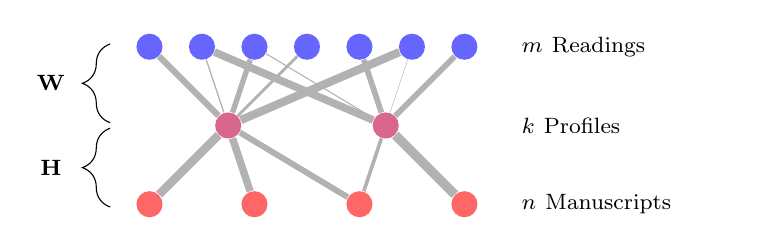
\begin{tikzpicture}
				%Readings-Texttypes-MSS graph:
				%Readings:
				\path
					(0.0, 2) node[shape=circle, fill=blue!60, scale=1.0 ](rtm_r1) {}
					(0.6666, 2) node[shape=circle, fill=blue!60, scale=1.0 ](rtm_r2) {}
					(1.3333, 2) node[shape=circle, fill=blue!60, scale=1.0 ](rtm_r3) {}
					(2.0, 2) node[shape=circle, fill=blue!60, scale=1.0 ](rtm_r4) {}
					(2.6666, 2) node[shape=circle, fill=blue!60, scale=1.0 ](rtm_r5) {}
					(3.3333, 2) node[shape=circle, fill=blue!60, scale=1.0 ](rtm_r6) {}
					(4.0, 2) node[shape=circle, fill=blue!60, scale=1.0 ](rtm_r7) {};
				%Profiles:
				\path
					(1.0, 1) node[shape=circle, fill=purple!60, scale=1.0 ](rtm_t1) {}
					(3.0, 1) node[shape=circle, fill=purple!60, scale=1.0 ](rtm_t2) {};
				%MSS:
				\path
					(0.0, 0) node[shape=circle, fill=red!60, scale=1.0 ](rtm_m1) {}
					(1.3333, 0) node[shape=circle, fill=red!60, scale=1.0 ](rtm_m2) {}
					(2.6666, -0) node[shape=circle, fill=red!60, scale=1.0 ](rtm_m3) {}
					(4.0, 0) node[shape=circle, fill=red!60, scale=1.0 ](rtm_m4) {};
				%Edges:
				%Reading-to-profile:
				\draw[line width=0.0768cm, color=black!30] (rtm_r1) -- (rtm_t1);
				\draw[line width=0.0158cm, color=black!30] (rtm_r2) -- (rtm_t1);
				\draw[line width=0.0974cm, color=black!30] (rtm_r2) -- (rtm_t2);
				\draw[line width=0.0679cm, color=black!30] (rtm_r3) -- (rtm_t1);
				\draw[line width=0.0136cm, color=black!30] (rtm_r3) -- (rtm_t2);
				\draw[line width=0.0357cm, color=black!30] (rtm_r4) -- (rtm_t1);
				\draw[line width=0.0728cm, color=black!30] (rtm_r5) -- (rtm_t2);
				\draw[line width=0.1047cm, color=black!30] (rtm_r6) -- (rtm_t1);
				\draw[line width=0.0058cm, color=black!30] (rtm_r6) -- (rtm_t2);
				\draw[line width=0.0728cm, color=black!30] (rtm_r7) -- (rtm_t2);
				%Profile-to-MS:
				\draw[line width=0.1085cm, color=black!30] (rtm_t1) -- (rtm_m1);
				\draw[line width=0.0945cm, color=black!30] (rtm_t1) -- (rtm_m2);
				\draw[line width=0.0758cm, color=black!30] (rtm_t1) -- (rtm_m3);
				\draw[line width=0.0461cm, color=black!30] (rtm_t2) -- (rtm_m3);
				\draw[line width=0.1197cm, color=black!30] (rtm_t2) -- (rtm_m4);
				%Labels:
				\draw 
					(6.0, 2) node[text width=1in, align=left] (rtm_rl) {\footnotesize $m$ Readings}
					(6.0, 1) node[text width=1in, align=left] (rtm_tl) {\footnotesize $k$ Profiles}
					(6.0, 0) node[text width=1in, align=left] (rtm_ml) {\footnotesize $n$ Manuscripts};
				\draw [decorate,decoration={brace,amplitude=10pt},xshift=-0.5cm,yshift=1pt]
						(0.0,1.0) -- (0.0,2.0) node [midway,xshift=-0.75cm] {\footnotesize $\mathbf{W}$};
				\draw [decorate,decoration={brace,amplitude=10pt},xshift=-0.5cm,yshift=-1pt]
						(0.0,0.0) -- (0.0,1.0) node [midway,xshift=-0.75cm] {\footnotesize $\mathbf{H}$};
				\end{tikzpicture}
			\end{center}
			...to reconstruct the large set of original relationships
			\begin{center}
				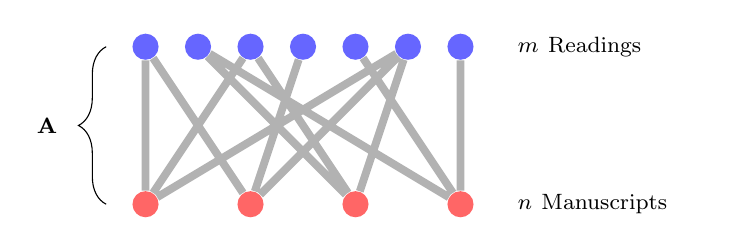
\begin{tikzpicture}
					%Readings-MSS graph:
					%Readings:
					\path
						(0.0, 2) node[shape=circle, fill=blue!60, scale=1.0 ](rm_r1) {}
						(0.6666, 2) node[shape=circle, fill=blue!60, scale=1.0 ](rm_r2) {}
						(1.3333, 2) node[shape=circle, fill=blue!60, scale=1.0 ](rm_r3) {}
						(2.0, 2) node[shape=circle, fill=blue!60, scale=1.0 ](rm_r4) {}
						(2.6666, 2) node[shape=circle, fill=blue!60, scale=1.0 ](rm_r5) {}
						(3.3333, 2) node[shape=circle, fill=blue!60, scale=1.0 ](rm_r6) {}
						(4.0, 2) node[shape=circle, fill=blue!60, scale=1.0 ](rm_r7) {};
					%MSS:
					\path
						(0.0, 0) node[shape=circle, fill=red!60, scale=1.0 ](rm_m1) {}
						(1.3333, 0) node[shape=circle, fill=red!60, scale=1.0 ](rm_m2) {}
						(2.6666, 0) node[shape=circle, fill=red!60, scale=1.0 ](rm_m3) {}
						(4.0, 0) node[shape=circle, fill=red!60, scale=1.0 ](rm_m4) {};
					%Edges:
					\draw[line width=0.1cm, color=black!30]
						(rm_r1) -- (rm_m1)
						(rm_r1) -- (rm_m2)
						(rm_r2) -- (rm_m3)
						(rm_r2) -- (rm_m4)
						(rm_r3) -- (rm_m1)
						(rm_r3) -- (rm_m3)
						(rm_r4) -- (rm_m2)
						(rm_r5) -- (rm_m4)
						(rm_r6) -- (rm_m1)
						(rm_r6) -- (rm_m2)
						(rm_r6) -- (rm_m3)
						(rm_r7) -- (rm_m4);
					%Labels:
					\draw 
						(6.0, 2) node[text width=1in, align=left] (rtm_rl) {\footnotesize $m$ Readings}
						(6.0, 0) node[text width=1in, align=left] (rtm_ml) {\footnotesize $n$ Manuscripts};
					\draw [decorate,decoration={brace,amplitude=10pt},xshift=-0.5cm,yshift=0pt]
						(0.0,0.0) -- (0.0,2.0) node [midway,xshift=-0.75cm] {\footnotesize $\mathbf{A}$};
				\end{tikzpicture}
			\end{center}
		\end{itemize}
	\end{frame}
	\begin{frame}{Non-negative Matrix Factorization}
		\begin{itemize}
			\item The process:
			\begin{enumerate}
				\item Start with guesses for $\mathbf{W}$ and $\mathbf{H}$
				\item Fix $\mathbf{W}$, optimize the weights in $\mathbf{H}$\hfill(Quantitative Method)
				\item Fix $\mathbf{H}$, optimize the weights in $\mathbf{W}$\hfill(Claremont Profile Method)
				\item Repeat steps 2 and 3 until the difference between $\mathbf{A}$ and $\mathbf{W}\mathbf{H}$ no longer decreases
			\end{enumerate}
			\begin{center}
				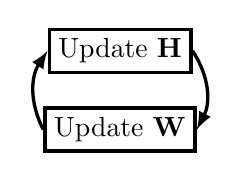
\begin{tikzpicture}
					%Nodes:
					\node[rectangle, align=center, fill=white, draw, very thick] (h)  at (0, 1) {Update $\mathbf{H}$};
					\node[rectangle, align=center, fill=white, draw, very thick] (w) at (0, 0) {Update $\mathbf{W}$};
					%Edges:
					\draw[->, >=latex, very thick] (h.east) to[bend left] (w.east);
					\draw[->, >=latex, very thick] (w.west) to[bend left] (h.west);
				\end{tikzpicture}
			\end{center}
			\item Guaranteed to terminate with \emph{locally optimal} groupings in $\mathbf{W}$ and $\mathbf{H}$\footnote{\cite{GS00}.}
		\end{itemize}
	\end{frame}
	\begin{frame}{Results: Jude}
		\begin{itemize}
			\item Tommy Wasserman's collation of Jude contains $1346$ variant readings and $560$ manuscripts (including lectionaries)\footnote{\cite{Wasserman06}.}
			\item Filtering out $42$ fragmentary manuscripts ($< 300$ known readings) yields a matrix $\mathbf{A}$ with $m = 1346$ rows and $n = 518$ columns
			\item The fragmentary manuscripts can be classified after groups are established\footnote{For details, see the appendix of \cite{McCollum19}.}
		\end{itemize}
	\end{frame}
	\begin{frame}{Results: Jude}
		\begin{itemize}
			\item We select the number of profiles $k$ based on several factors:
			\begin{itemize}
				\item Overlap of readings in profiles
				\item Mixture of profiles in manuscripts
				\item Consistency of manuscript groupings when random starting points are used (the \emph{cophenetic correlation coefficient})\footnote{\cite{BTGM04}.}
			\end{itemize}
			\begin{center}
				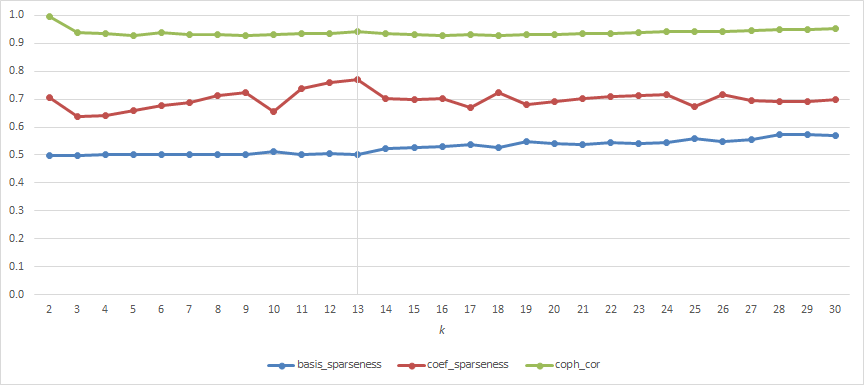
\includegraphics[width=0.90\textwidth]{../graphics/jude_uniform_rank_est.png}
			\end{center}
		\end{itemize}
	\end{frame}
	\begin{frame}{Results: Jude}
		\begin{itemize}
			\item The $k = 13$ groups identified by NMF correspond to groups in the Catholic Epistles identified in the literature
			\begin{center}
				\matrixfont
				\footnotesize
				\begin{tabular}{p{2.5in}p{1.25in}}
					Members (by Gregory-Aland number) & Group\\
					\hline
					920, 1277, 1859, 1719, 452, 1857, 1871, 941, 1103, 1352, etc. & Κ (von Soden)\\
					\hline
					141, 204, 394, 444, 1101, 1723, 1737, 1752, 1865, 2221, etc. & Κ\textsuperscript{r} (von Soden)\\
					\hline
					390, 1863, 912, 234, 1861, 2085, 1753, 2279, 42, 996, etc. & Κ\textsuperscript{c} (von Soden)\\
					\hline
					L606, L938, L145, L840, L740, L2106, L2394, L809, L1279, L62, etc. & Lectionary (Colwell)\\
					\hline
					606, 454, 641, 103, 221, 2125, 314, 250, 1888, 393, etc. & Ο, Θδ Commentaries (von Soden)\\
					\hline
					619, 1780, 1175, 330, 1769, 2516, 917, 451, 1162, 601, etc. & \emph{f}\textsuperscript{1780} (unidentified)\\
					\hline
					1563, 1718, 1425, 1359, 1066, 0142, 056 & \emph{f}\textsuperscript{0142} (unidentified)
				\end{tabular}
			\end{center}
		\end{itemize}
	\end{frame}
	\begin{frame}{Results: Jude}
		\begin{itemize}
			\item The $k = 13$ groups identified by NMF correspond to groups in the Catholic Epistles identified in the literature
			\begin{center}
				\matrixfont
				\footnotesize
				\begin{tabular}{p{2.5in}p{1.25in}}
					Members (by Gregory-Aland number) & Group\\
					\hline
					03, 623, $\mathfrak{P}$\textsuperscript{72}, 81, 5, 326, 33, 1837, 93, 665, etc. & Η (von Soden)\\
					\hline
					321, 918, 307, 453, 2197, 2818, 1678, 94, 2186, 1840, etc. & \emph{f}\textsuperscript{453} (Spencer, Wachtel,\newline Howe)\\
					\hline
					323, 1241, 322, 1739, 1881, 2298, 6 & \emph{f}\textsuperscript{1739} (Zuntz, Geer)\\
					\hline
					1505, 2495, 1611, 1292, 630, 2200, 1765, 1832, 2494, 876, etc. & \emph{f}\textsuperscript{2138}/Harklean\newline (Amphoux)\\
					\hline
					1843, 1869, 506, 1903, 489, 927, 203, 1868, 1729, 1873, etc. & Ι (von Soden)\\
					\hline
					915, 88, 459, 104, 1846, 1838, 1842, 1845 & \emph{f}\textsuperscript{915} (unidentified)
				\end{tabular}
			\end{center}
		\end{itemize}
	\end{frame}
	\begin{frame}{Results: John 18}
		\begin{itemize}
			\item Applying NMF to Morrill's collation of all continuous-text manuscripts of John 18 illustrates some of the idiosyncrasies of the method and how to deal with them\footnote{\cite{Morrill12}.}
			\item Significantly larger and more ``square'' collation: $m = 1545$ variant readings and $n = 1610$ manuscripts after filtering out fragmentary manuscripts (< $350$ known readings)
			\item (Recall that the collation matrix for Jude was $1346 \times 518$)
		\end{itemize}
	\end{frame}
	\begin{frame}{Results: John 18}
		\begin{itemize}
			\item Applying NMF to the matrix as-is separates readings common to multiple groups into their own ``core'' profiles
			\item No manuscripts belong to these profiles, but many appear ``mixed'' with it
			\item Symptom of volume and similarity of manuscripts, especially Byzantine ones
		\end{itemize}
		\begin{center}
			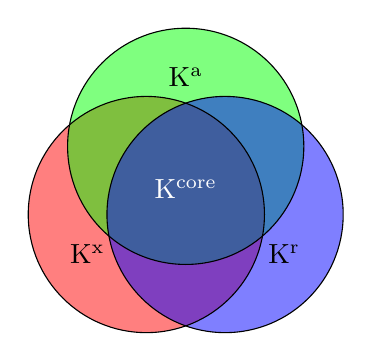
\begin{tikzpicture}
				\begin{scope}[fill opacity=0.5]
					\fill[red] (0,0) circle (1.5cm);
					\fill[green] (60:1cm) circle (1.5cm);
					\fill[blue] (0:1cm) circle (1.5cm);
					\draw (0,0) circle (1.5cm) node[below] {};
					\draw (60:1cm) circle (1.5cm) node [above] {};
					\draw (0:1cm) circle (1.5cm) node [below] {};
					\draw (-0.75,-0.5) node[opacity=1.0] {\matrixfont K\textsuperscript{x}};
					\draw (0.5,1.75) node[opacity=1.0] {\matrixfont K\textsuperscript{a}};
					\draw (1.75,-0.5) node[opacity=1.0] {\matrixfont K\textsuperscript{r}};
					\draw (0.5,0.325) node[white, opacity=1.0] {\matrixfont K\textsuperscript{core}};
				\end{scope}
			\end{tikzpicture}
		\end{center}
	\end{frame}
	\begin{frame}{Results: John 18}
		\begin{itemize}
			\item To remedy this, weigh readings in the original matrix by their \emph{inverse document frequency} (IDF)\footnote{\cite{Jones72}.}
			\begin{equation*}
				\log\frac{\mathit{n}}{\#\{\mathrm{MSS\ with\ reading}\}}
			\end{equation*}
			\item Removing singular readings is helpful in this setting
			\item Encourages NMF to isolate unique group readings in profiles
		\end{itemize}
		\begin{center}
			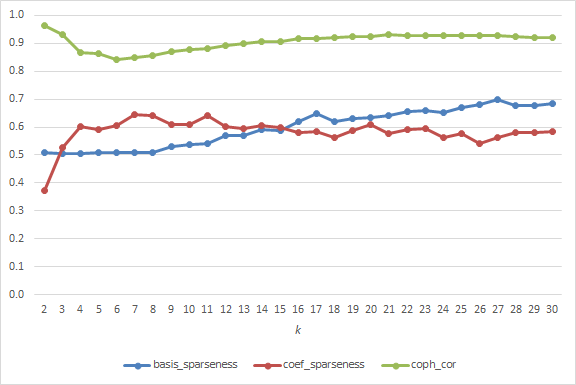
\includegraphics[width=0.45\textwidth]{../graphics/john_18_uniform_rank_est.png}
			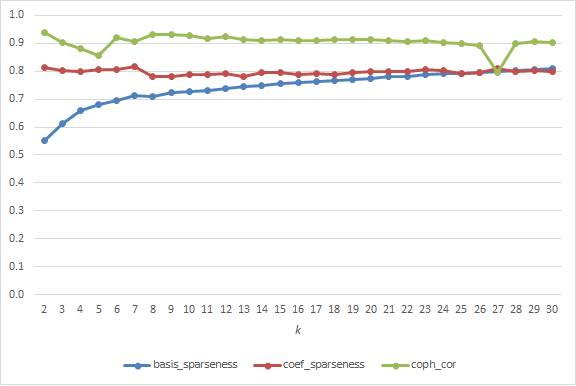
\includegraphics[width=0.45\textwidth]{../graphics/john_18_idf_rank_est.png}
			\begin{tabular}{c @{\hskip 1.25in} c}
				No weighting & IDF weighting
			\end{tabular}
		\end{center}
	\end{frame}
	\begin{frame}{Results: John 18}
		\begin{itemize}
			\item With $k = 12$, NMF identifies known groups from the literature
			\begin{center}
				\matrixfont
				\footnotesize
				\begin{tabular}{p{2.5in}p{0.75in}}
					Members (by Gregory-Aland number) & Group\\
					\hline
					2605, 492, 1215, 2897, 1090, 1567, 1210, 851, 494, 2406, etc. & Κ\textsuperscript{x} (von Soden)\\
					\hline
					47, 1126, 61, 1138, 58, 56, 189, 1236, 825, 1614, etc. & Κ\textsuperscript{r} (von Soden)\\
					\hline
					2902, 1219, 1079, 489, 114, 2404, 389, 2193, 699, 1627, etc. & Κ\textsuperscript{a} (von Soden)\\
					\hline
					1534, 741, 857, 744, 2735, 1160, 817, 1261, 2470, 833, etc. & Θε Commentaries (von Soden)\\
					\hline
					892, 977, 555, 16, 152, 513, 1243, 829, 348, 1579, etc. & \emph{f}\textsuperscript{16}+\emph{f}\textsuperscript{1216} (Wisse)\\
					\hline
					1663, 1413, 2291, 86, 569, 71, 1170, 1014, 1531, 2705, etc. & M27+Cl1531 (Wisse)
				\end{tabular}
			\end{center}
		\end{itemize}
	\end{frame}
	\begin{frame}{Results: John 18}
		\begin{itemize}
			\item With $k = 12$, NMF identifies known groups from the literature
			\begin{center}
				\matrixfont
				\footnotesize
				\begin{tabular}{p{2.5in}p{1.25in}}
					Members (by Gregory-Aland number) & Group\\
					\hline
					01, 032, 05, 579, 1654, 2561, 1242 & Egyptian\\
					\hline
					1820, 2129, 865, 033, 019, 1819, 213, 03, 33, 1321, etc. & Alexandrian\\
					\hline
					1, 1582, 357, 138, 565, 209, 994, 2713, 2575, 1784, etc. & \emph{f}\textsuperscript{1} (Lake)\\
					\hline
					13, 788, 826, 828, 543, 69, 346, 1689, 124, 2786, etc. & \emph{f}\textsuperscript{13} (Lake and Lake, Geerlings)\\
					\hline
					2524, 1001, 1268, 2397, 352, 2728, 132, 175, 1701, 2252, etc. & Cl1001+Cl352 (Wisse)\\
					\hline
					1446, 1050, 706, 1457, 827, 2620, 1128, 0211, 2707, 1402, etc. & Cl827 (Wisse)
				\end{tabular}
			\end{center}
		\end{itemize}
	\end{frame}
	\begin{frame}{Concluding Observations}
		\begin{columns}[T]
			\begin{column}{0.6\textwidth}
				\begin{itemize}
					\item In John 18, Gregory-Aland 03 (Codex Vaticanus, B) stands out as an instructive example
					\item Appears to be mixed between the ``Egyptian'' and ``Alexandrian'' profiles, but could preserve a text earlier than both
				\end{itemize}
			\end{column}
			\begin{column}{0.3\textwidth}
				\begin{center}
					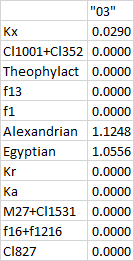
\includegraphics[width=0.5\textwidth]{../graphics/john_18_03_coefs.png}
				\end{center}
			\end{column}
		\end{columns}
		\begin{itemize}
			\item NMF identifies relationships, but not their directions
			\item Pre-genealogical, but not genealogical
		\end{itemize}
		\begin{center}
			\begin{tikzpicture}
				%Nodes
				\path
					(-1.0, 1) node[shape=circle](ms_1) {1}
					(0.0, 0) node[shape=circle](ms_2) {2}
					(2.0, 0) node[shape=circle](ms_3) {3};
				%Edges
				\draw[draw]
					(0,2) -- (ms_1)
					(0,2) -- (1,1)
					(1,1) -- (ms_2)
					(1,1) -- (ms_3);
				%Edge markings
				\draw[draw,decoration={markings, mark=at position .5  with {\node[transform shape] {|};}}] 
				(0,2) edge[decorate] (ms_1);
				\draw[draw,decoration={markings, mark=at position .5  with {\node[transform shape] {|||};}}] 
				(0,2) edge[decorate] (1,1);
				\draw[draw,decoration={markings, mark=at position .5  with {\node[transform shape] {};}}] 
				(1,1) edge[decorate] (ms_2);
				\draw[draw,decoration={markings, mark=at position .5  with {\node[transform shape] {|};}}] 
				(1,1) edge[decorate] (ms_3);
				%Cluster cloud
				\node[cloud, cloud puffs=13, cloud ignores aspect, minimum width=3cm, minimum height=2cm, align=center,fill=white, draw, very thick] (cluster)  at (6, 1) {{\large\bf 2}\hspace{0.5cm}{\normalsize\bf 3}\hspace{0.5cm}{\small 1}};
				%Arrow
				\draw[->, >=latex, line width=0.25cm] (2.5,1) -- (4,1);
			\end{tikzpicture}
		\end{center}
	\end{frame}
	\begin{frame}{Concluding Observations}
		\begin{itemize}
			\item The advantage: few assumptions and editorial decisions are required
			\item Intended for use in ``pre-processing'' (manuscript and test reading selection)
			\item Useful for other applications (new manuscript classification)
			\item Work in progress: applying NMF to \textasciitilde 2000 manuscripts in the \emph{pericope adulterae} (with Maurice A. Robinson)
		\end{itemize}
	\end{frame}
	\begin{frame}[allowframebreaks]
		\printbibliography
	\end{frame}
\end{document}